\documentclass[1p]{elsarticle_modified}
%\bibliographystyle{elsarticle-num}

%\usepackage[colorlinks]{hyperref}
%\usepackage{abbrmath_seonhwa} %\Abb, \Ascr, \Acal ,\Abf, \Afrak
\usepackage{amsfonts}
\usepackage{amssymb}
\usepackage{amsmath}
\usepackage{amsthm}
\usepackage{scalefnt}
\usepackage{amsbsy}
\usepackage{kotex}
\usepackage{caption}
\usepackage{subfig}
\usepackage{color}
\usepackage{graphicx}
\usepackage{xcolor} %% white, black, red, green, blue, cyan, magenta, yellow
\usepackage{float}
\usepackage{setspace}
\usepackage{hyperref}

\usepackage{tikz}
\usetikzlibrary{arrows}

\usepackage{multirow}
\usepackage{array} % fixed length table
\usepackage{hhline}

%%%%%%%%%%%%%%%%%%%%%
\makeatletter
\renewcommand*\env@matrix[1][\arraystretch]{%
	\edef\arraystretch{#1}%
	\hskip -\arraycolsep
	\let\@ifnextchar\new@ifnextchar
	\array{*\c@MaxMatrixCols c}}
\makeatother %https://tex.stackexchange.com/questions/14071/how-can-i-increase-the-line-spacing-in-a-matrix
%%%%%%%%%%%%%%%

\usepackage[normalem]{ulem}

\newcommand{\msout}[1]{\ifmmode\text{\sout{\ensuremath{#1}}}\else\sout{#1}\fi}
%SOURCE: \msout is \stkout macro in https://tex.stackexchange.com/questions/20609/strikeout-in-math-mode

\newcommand{\cancel}[1]{
	\ifmmode
	{\color{red}\msout{#1}}
	\else
	{\color{red}\sout{#1}}
	\fi
}

\newcommand{\add}[1]{
	{\color{blue}\uwave{#1}}
}

\newcommand{\replace}[2]{
	\ifmmode
	{\color{red}\msout{#1}}{\color{blue}\uwave{#2}}
	\else
	{\color{red}\sout{#1}}{\color{blue}\uwave{#2}}
	\fi
}

\newcommand{\Sol}{\mathcal{S}} %segment
\newcommand{\D}{D} %diagram
\newcommand{\A}{\mathcal{A}} %arc


%%%%%%%%%%%%%%%%%%%%%%%%%%%%%5 test

\def\sl{\operatorname{\textup{SL}}(2,\Cbb)}
\def\psl{\operatorname{\textup{PSL}}(2,\Cbb)}
\def\quan{\mkern 1mu \triangleright \mkern 1mu}

\theoremstyle{definition}
\newtheorem{thm}{Theorem}[section]
\newtheorem{prop}[thm]{Proposition}
\newtheorem{lem}[thm]{Lemma}
\newtheorem{ques}[thm]{Question}
\newtheorem{cor}[thm]{Corollary}
\newtheorem{defn}[thm]{Definition}
\newtheorem{exam}[thm]{Example}
\newtheorem{rmk}[thm]{Remark}
\newtheorem{alg}[thm]{Algorithm}

\newcommand{\I}{\sqrt{-1}}
\begin{document}

%\begin{frontmatter}
%
%\title{Boundary parabolic representations of knots up to 8 crossings}
%
%%% Group authors per affiliation:
%\author{Yunhi Cho} 
%\address{Department of Mathematics, University of Seoul, Seoul, Korea}
%\ead{yhcho@uos.ac.kr}
%
%
%\author{Seonhwa Kim} %\fnref{s_kim}}
%\address{Center for Geometry and Physics, Institute for Basic Science, Pohang, 37673, Korea}
%\ead{ryeona17@ibs.re.kr}
%
%\author{Hyuk Kim}
%\address{Department of Mathematical Sciences, Seoul National University, Seoul 08826, Korea}
%\ead{hyukkim@snu.ac.kr}
%
%\author{Seokbeom Yoon}
%\address{Department of Mathematical Sciences, Seoul National University, Seoul, 08826,  Korea}
%\ead{sbyoon15@snu.ac.kr}
%
%\begin{abstract}
%We find all boundary parabolic representation of knots up to 8 crossings.
%
%\end{abstract}
%\begin{keyword}
%    \MSC[2010] 57M25 
%\end{keyword}
%
%\end{frontmatter}

%\linenumbers
%\tableofcontents
%
\newcommand\colored[1]{\textcolor{white}{\rule[-0.35ex]{0.8em}{1.4ex}}\kern-0.8em\color{red} #1}%
%\newcommand\colored[1]{\textcolor{white}{ #1}\kern-2.17ex	\textcolor{white}{ #1}\kern-1.81ex	\textcolor{white}{ #1}\kern-2.15ex\color{red}#1	}

{\Large $\underline{12a_{1174}~(K12a_{1174})}$}

\setlength{\tabcolsep}{10pt}
\renewcommand{\arraystretch}{1.6}
\vspace{1cm}\begin{tabular}{m{100pt}>{\centering\arraybackslash}m{274pt}}
\multirow{5}{120pt}{
	\centering
	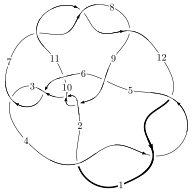
\includegraphics[width=112pt]{../../../GIT/diagram.site/Diagrams/png/1975_12a_1174.png}\\
\ \ \ A knot diagram\footnotemark}&
\allowdisplaybreaks
\textbf{Linearized knot diagam} \\
\cline{2-2}
 &
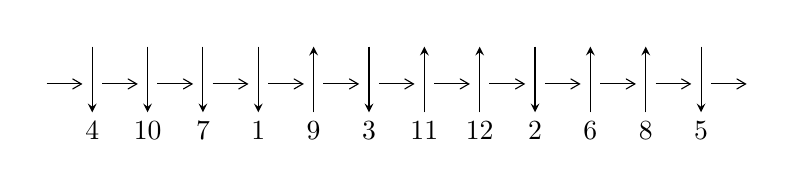
\begin{tikzpicture}[x=20pt, y=17pt]
	% nodes
	\node (C0) at (0, 0) {};
	\node (C1) at (1, 0) {};
	\node (C1U) at (1, +1) {};
	\node (C1D) at (1, -1) {4};

	\node (C2) at (2, 0) {};
	\node (C2U) at (2, +1) {};
	\node (C2D) at (2, -1) {10};

	\node (C3) at (3, 0) {};
	\node (C3U) at (3, +1) {};
	\node (C3D) at (3, -1) {7};

	\node (C4) at (4, 0) {};
	\node (C4U) at (4, +1) {};
	\node (C4D) at (4, -1) {1};

	\node (C5) at (5, 0) {};
	\node (C5U) at (5, +1) {};
	\node (C5D) at (5, -1) {9};

	\node (C6) at (6, 0) {};
	\node (C6U) at (6, +1) {};
	\node (C6D) at (6, -1) {3};

	\node (C7) at (7, 0) {};
	\node (C7U) at (7, +1) {};
	\node (C7D) at (7, -1) {11};

	\node (C8) at (8, 0) {};
	\node (C8U) at (8, +1) {};
	\node (C8D) at (8, -1) {12};

	\node (C9) at (9, 0) {};
	\node (C9U) at (9, +1) {};
	\node (C9D) at (9, -1) {2};

	\node (C10) at (10, 0) {};
	\node (C10U) at (10, +1) {};
	\node (C10D) at (10, -1) {6};

	\node (C11) at (11, 0) {};
	\node (C11U) at (11, +1) {};
	\node (C11D) at (11, -1) {8};

	\node (C12) at (12, 0) {};
	\node (C12U) at (12, +1) {};
	\node (C12D) at (12, -1) {5};
	\node (C13) at (13, 0) {};

	% arrows
	\draw[->,>={angle 60}]
	(C0) edge (C1) (C1) edge (C2) (C2) edge (C3) (C3) edge (C4) (C4) edge (C5) (C5) edge (C6) (C6) edge (C7) (C7) edge (C8) (C8) edge (C9) (C9) edge (C10) (C10) edge (C11) (C11) edge (C12) (C12) edge (C13) ;	\draw[->,>=stealth]
	(C1U) edge (C1D) (C2U) edge (C2D) (C3U) edge (C3D) (C4U) edge (C4D) (C5D) edge (C5U) (C6U) edge (C6D) (C7D) edge (C7U) (C8D) edge (C8U) (C9U) edge (C9D) (C10D) edge (C10U) (C11D) edge (C11U) (C12U) edge (C12D) ;
	\end{tikzpicture} \\
\hhline{~~} \\& 
\textbf{Solving Sequence} \\ \cline{2-2} 
 &
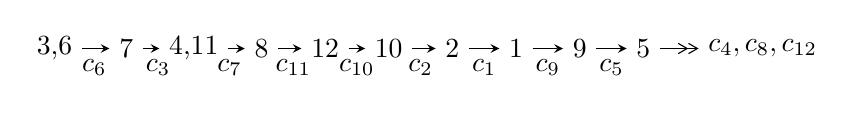
\begin{tikzpicture}[x=23pt, y=7pt]
	% node
	\node (A0) at (-1/8, 0) {3,6};
	\node (A1) at (1, 0) {7};
	\node (A2) at (33/16, 0) {4,11};
	\node (A3) at (25/8, 0) {8};
	\node (A4) at (33/8, 0) {12};
	\node (A5) at (41/8, 0) {10};
	\node (A6) at (49/8, 0) {2};
	\node (A7) at (57/8, 0) {1};
	\node (A8) at (65/8, 0) {9};
	\node (A9) at (73/8, 0) {5};
	\node (C1) at (1/2, -1) {$c_{6}$};
	\node (C2) at (3/2, -1) {$c_{3}$};
	\node (C3) at (21/8, -1) {$c_{7}$};
	\node (C4) at (29/8, -1) {$c_{11}$};
	\node (C5) at (37/8, -1) {$c_{10}$};
	\node (C6) at (45/8, -1) {$c_{2}$};
	\node (C7) at (53/8, -1) {$c_{1}$};
	\node (C8) at (61/8, -1) {$c_{9}$};
	\node (C9) at (69/8, -1) {$c_{5}$};
	\node (A10) at (11, 0) {$c_{4},c_{8},c_{12}$};

	% edge
	\draw[->,>=stealth]	
	(A0) edge (A1) (A1) edge (A2) (A2) edge (A3) (A3) edge (A4) (A4) edge (A5) (A5) edge (A6) (A6) edge (A7) (A7) edge (A8) (A8) edge (A9) ;
	\draw[->>,>={angle 60}]	
	(A9) edge (A10);
\end{tikzpicture} \\ 

\end{tabular} \\

\footnotetext{
The image of knot diagram is generated by the software ``\textbf{Draw programme}" developed by Andrew Bartholomew(\url{http://www.layer8.co.uk/maths/draw/index.htm\#Running-draw}), where we modified some parts for our purpose(\url{https://github.com/CATsTAILs/LinksPainter}).
}\phantom \\ \newline 
\centering \textbf{Ideals for irreducible components\footnotemark of $X_{\text{par}}$} 
 
\begin{align*}
I^u_{1}&=\langle 
-1.79172\times10^{293} u^{92}+5.18538\times10^{293} u^{91}+\cdots+5.07764\times10^{292} b+2.25779\times10^{296},\\
\phantom{I^u_{1}}&\phantom{= \langle  }-2.37870\times10^{296} u^{92}+7.02532\times10^{296} u^{91}+\cdots+5.48893\times10^{295} a+2.78497\times10^{299},\\
\phantom{I^u_{1}}&\phantom{= \langle  }u^{93}-2 u^{92}+\cdots+2191 u-1081\rangle \\
I^u_{2}&=\langle 
-32320 u^{20}+116817 u^{19}+\cdots+14919 b-48202,\;12963 u^{20}+67496 u^{19}+\cdots+14919 a-214943,\\
\phantom{I^u_{2}}&\phantom{= \langle  }u^{21}-3 u^{20}+\cdots- u+1\rangle \\
\\
\end{align*}
\raggedright * 2 irreducible components of $\dim_{\mathbb{C}}=0$, with total 114 representations.\\
\footnotetext{All coefficients of polynomials are rational numbers. But the coefficients are sometimes approximated in decimal forms when there is not enough margin.}
\newpage
\renewcommand{\arraystretch}{1}
\centering \section*{I. $I^u_{1}= \langle -1.79\times10^{293} u^{92}+5.19\times10^{293} u^{91}+\cdots+5.08\times10^{292} b+2.26\times10^{296},\;-2.38\times10^{296} u^{92}+7.03\times10^{296} u^{91}+\cdots+5.49\times10^{295} a+2.78\times10^{299},\;u^{93}-2 u^{92}+\cdots+2191 u-1081 \rangle$}
\flushleft \textbf{(i) Arc colorings}\\
\begin{tabular}{m{7pt} m{180pt} m{7pt} m{180pt} }
\flushright $a_{3}=$&$\begin{pmatrix}0\\u\end{pmatrix}$ \\
\flushright $a_{6}=$&$\begin{pmatrix}1\\0\end{pmatrix}$ \\
\flushright $a_{7}=$&$\begin{pmatrix}1\\u^2\end{pmatrix}$ \\
\flushright $a_{4}=$&$\begin{pmatrix}- u\\- u^3+u\end{pmatrix}$ \\
\flushright $a_{11}=$&$\begin{pmatrix}4.33363 u^{92}-12.7991 u^{91}+\cdots+15938.8 u-5073.80\\3.52865 u^{92}-10.2122 u^{91}+\cdots+14118.3 u-4446.54\end{pmatrix}$ \\
\flushright $a_{8}=$&$\begin{pmatrix}-0.294962 u^{92}+0.652560 u^{91}+\cdots-3271.15 u+901.397\\-2.28531 u^{92}+6.61498 u^{91}+\cdots-9727.95 u+3065.58\end{pmatrix}$ \\
\flushright $a_{12}=$&$\begin{pmatrix}1.38877 u^{92}-3.49286 u^{91}+\cdots+5890.99 u-1513.44\\-1.10004 u^{92}+3.10829 u^{91}+\cdots-5830.00 u+1865.50\end{pmatrix}$ \\
\flushright $a_{10}=$&$\begin{pmatrix}0.804989 u^{92}-2.58688 u^{91}+\cdots+1820.44 u-627.253\\3.52865 u^{92}-10.2122 u^{91}+\cdots+14118.3 u-4446.54\end{pmatrix}$ \\
\flushright $a_{2}=$&$\begin{pmatrix}-1.54792 u^{92}+4.79711 u^{91}+\cdots-4518.22 u+1695.55\\0.788795 u^{92}-2.14540 u^{91}+\cdots+3223.00 u-926.289\end{pmatrix}$ \\
\flushright $a_{1}=$&$\begin{pmatrix}-1.06239 u^{92}+3.58010 u^{91}+\cdots-2164.67 u+1046.92\\0.454016 u^{92}-1.20759 u^{91}+\cdots+1933.22 u-543.550\end{pmatrix}$ \\
\flushright $a_{9}=$&$\begin{pmatrix}1.40660 u^{92}-3.76007 u^{91}+\cdots+7861.74 u-2444.89\\1.43867 u^{92}-4.20929 u^{91}+\cdots+5481.94 u-1756.79\end{pmatrix}$ \\
\flushright $a_{5}=$&$\begin{pmatrix}-1.81351 u^{92}+5.12931 u^{91}+\cdots-6832.74 u+2194.88\\2.31351 u^{92}-6.77939 u^{91}+\cdots+8527.69 u-2737.03\end{pmatrix}$\\&\end{tabular}
\flushleft \textbf{(ii) Obstruction class $= -1$}\\~\\
\flushleft \textbf{(iii) Cusp Shapes $= 1.43488 u^{92}-3.65079 u^{91}+\cdots+6204.45 u-1887.76$}\\~\\
\newpage\renewcommand{\arraystretch}{1}
\flushleft \textbf{(iv) u-Polynomials at the component}\newline \\
\begin{tabular}{m{50pt}|m{274pt}}
Crossings & \hspace{64pt}u-Polynomials at each crossing \\
\hline $$\begin{aligned}c_{1},c_{4},c_{12}\end{aligned}$$&$\begin{aligned}
&u^{93}-3 u^{92}+\cdots+12 u-1
\end{aligned}$\\
\hline $$\begin{aligned}c_{2},c_{9}\end{aligned}$$&$\begin{aligned}
&u^{93}-34 u^{91}+\cdots-4634 u+2071
\end{aligned}$\\
\hline $$\begin{aligned}c_{3},c_{6}\end{aligned}$$&$\begin{aligned}
&u^{93}-2 u^{92}+\cdots+2191 u-1081
\end{aligned}$\\
\hline $$\begin{aligned}c_{5}\end{aligned}$$&$\begin{aligned}
&u^{93}-7 u^{92}+\cdots+245345 u+714407
\end{aligned}$\\
\hline $$\begin{aligned}c_{7},c_{8},c_{11}\end{aligned}$$&$\begin{aligned}
&u^{93}-7 u^{92}+\cdots-14 u-4
\end{aligned}$\\
\hline $$\begin{aligned}c_{10}\end{aligned}$$&$\begin{aligned}
&u^{93}+7 u^{91}+\cdots+21184 u-3499
\end{aligned}$\\
\hline
\end{tabular}\\~\\
\newpage\renewcommand{\arraystretch}{1}
\flushleft \textbf{(v) Riley Polynomials at the component}\newline \\
\begin{tabular}{m{50pt}|m{274pt}}
Crossings & \hspace{64pt}Riley Polynomials at each crossing \\
\hline $$\begin{aligned}c_{1},c_{4},c_{12}\end{aligned}$$&$\begin{aligned}
&y^{93}+95 y^{92}+\cdots+230 y-1
\end{aligned}$\\
\hline $$\begin{aligned}c_{2},c_{9}\end{aligned}$$&$\begin{aligned}
&y^{93}-68 y^{92}+\cdots+77411666 y-4289041
\end{aligned}$\\
\hline $$\begin{aligned}c_{3},c_{6}\end{aligned}$$&$\begin{aligned}
&y^{93}-58 y^{92}+\cdots+28900295 y-1168561
\end{aligned}$\\
\hline $$\begin{aligned}c_{5}\end{aligned}$$&$\begin{aligned}
&y^{93}-35 y^{92}+\cdots+27772503205947 y-510377361649
\end{aligned}$\\
\hline $$\begin{aligned}c_{7},c_{8},c_{11}\end{aligned}$$&$\begin{aligned}
&y^{93}-103 y^{92}+\cdots+1372 y-16
\end{aligned}$\\
\hline $$\begin{aligned}c_{10}\end{aligned}$$&$\begin{aligned}
&y^{93}+14 y^{92}+\cdots-580713924 y-12243001
\end{aligned}$\\
\hline
\end{tabular}\\~\\
\newpage\flushleft \textbf{(vi) Complex Volumes and Cusp Shapes}
$$\begin{array}{c|c|c}  
\text{Solutions to }I^u_{1}& \I (\text{vol} + \sqrt{-1}CS) & \text{Cusp shape}\\
 \hline 
\begin{aligned}
u &= -0.493220 + 0.865157 I \\
a &= \phantom{-}0.381752 - 0.204747 I \\
b &= \phantom{-}1.229960 - 0.447001 I\end{aligned}
 & \phantom{-}14.4991 - 4.6980 I & \phantom{-0.000000 } 0 \\ \hline\begin{aligned}
u &= -0.493220 - 0.865157 I \\
a &= \phantom{-}0.381752 + 0.204747 I \\
b &= \phantom{-}1.229960 + 0.447001 I\end{aligned}
 & \phantom{-}14.4991 + 4.6980 I & \phantom{-0.000000 } 0 \\ \hline\begin{aligned}
u &= -0.999193 + 0.206178 I \\
a &= -0.81805 + 1.25971 I \\
b &= \phantom{-}0.60869 + 1.28232 I\end{aligned}
 & -3.17135 + 0.93926 I & \phantom{-0.000000 } 0 \\ \hline\begin{aligned}
u &= -0.999193 - 0.206178 I \\
a &= -0.81805 - 1.25971 I \\
b &= \phantom{-}0.60869 - 1.28232 I\end{aligned}
 & -3.17135 - 0.93926 I & \phantom{-0.000000 } 0 \\ \hline\begin{aligned}
u &= -0.957998 + 0.358983 I \\
a &= -0.20807 + 1.83442 I \\
b &= \phantom{-}0.482838 + 0.488493 I\end{aligned}
 & \phantom{-}5.24104 + 4.96610 I & \phantom{-0.000000 } 0 \\ \hline\begin{aligned}
u &= -0.957998 - 0.358983 I \\
a &= -0.20807 - 1.83442 I \\
b &= \phantom{-}0.482838 - 0.488493 I\end{aligned}
 & \phantom{-}5.24104 - 4.96610 I & \phantom{-0.000000 } 0 \\ \hline\begin{aligned}
u &= \phantom{-}0.941539 + 0.247200 I \\
a &= \phantom{-}0.70673 - 1.39465 I \\
b &= -0.101345 - 0.424981 I\end{aligned}
 & \phantom{-}1.74388 - 1.76077 I & \phantom{-0.000000 } 0 \\ \hline\begin{aligned}
u &= \phantom{-}0.941539 - 0.247200 I \\
a &= \phantom{-}0.70673 + 1.39465 I \\
b &= -0.101345 + 0.424981 I\end{aligned}
 & \phantom{-}1.74388 + 1.76077 I & \phantom{-0.000000 } 0 \\ \hline\begin{aligned}
u &= \phantom{-}1.004200 + 0.244501 I \\
a &= \phantom{-}0.06367 - 1.54106 I \\
b &= \phantom{-}0.462032 - 0.656917 I\end{aligned}
 & -1.04854 - 3.13751 I & \phantom{-0.000000 } 0 \\ \hline\begin{aligned}
u &= \phantom{-}1.004200 - 0.244501 I \\
a &= \phantom{-}0.06367 + 1.54106 I \\
b &= \phantom{-}0.462032 + 0.656917 I\end{aligned}
 & -1.04854 + 3.13751 I & \phantom{-0.000000 } 0\\
 \hline 
 \end{array}$$\newpage$$\begin{array}{c|c|c}  
\text{Solutions to }I^u_{1}& \I (\text{vol} + \sqrt{-1}CS) & \text{Cusp shape}\\
 \hline 
\begin{aligned}
u &= \phantom{-}0.931604 + 0.243587 I \\
a &= -1.48753 + 2.26052 I \\
b &= -0.76730 + 1.22144 I\end{aligned}
 & \phantom{-}10.18600 + 4.17288 I & \phantom{-0.000000 } 0 \\ \hline\begin{aligned}
u &= \phantom{-}0.931604 - 0.243587 I \\
a &= -1.48753 - 2.26052 I \\
b &= -0.76730 - 1.22144 I\end{aligned}
 & \phantom{-}10.18600 - 4.17288 I & \phantom{-0.000000 } 0 \\ \hline\begin{aligned}
u &= -0.945716 + 0.448641 I \\
a &= -0.18841 + 1.50162 I \\
b &= -0.126174 + 1.037660 I\end{aligned}
 & \phantom{-}2.23609 + 2.02110 I & \phantom{-0.000000 } 0 \\ \hline\begin{aligned}
u &= -0.945716 - 0.448641 I \\
a &= -0.18841 - 1.50162 I \\
b &= -0.126174 - 1.037660 I\end{aligned}
 & \phantom{-}2.23609 - 2.02110 I & \phantom{-0.000000 } 0 \\ \hline\begin{aligned}
u &= -0.927769 + 0.198246 I \\
a &= \phantom{-}0.760639 + 0.112021 I \\
b &= -1.157820 + 0.065675 I\end{aligned}
 & \phantom{-}8.08998 - 0.30173 I & \phantom{-0.000000 } 0 \\ \hline\begin{aligned}
u &= -0.927769 - 0.198246 I \\
a &= \phantom{-}0.760639 - 0.112021 I \\
b &= -1.157820 - 0.065675 I\end{aligned}
 & \phantom{-}8.08998 + 0.30173 I & \phantom{-0.000000 } 0 \\ \hline\begin{aligned}
u &= -0.922638 + 0.013782 I \\
a &= \phantom{-}0.607351 - 1.268960 I \\
b &= \phantom{-}0.418728 - 0.759155 I\end{aligned}
 & -1.47830 + 0.09644 I & \phantom{-0.000000 } 0 \\ \hline\begin{aligned}
u &= -0.922638 - 0.013782 I \\
a &= \phantom{-}0.607351 + 1.268960 I \\
b &= \phantom{-}0.418728 + 0.759155 I\end{aligned}
 & -1.47830 - 0.09644 I & \phantom{-0.000000 } 0 \\ \hline\begin{aligned}
u &= \phantom{-}0.900637 + 0.166565 I \\
a &= \phantom{-}1.094280 + 0.849188 I \\
b &= \phantom{-}2.22704 + 0.89576 I\end{aligned}
 & \phantom{-}10.45250 - 5.98256 I & \phantom{-0.000000 } 0 \\ \hline\begin{aligned}
u &= \phantom{-}0.900637 - 0.166565 I \\
a &= \phantom{-}1.094280 - 0.849188 I \\
b &= \phantom{-}2.22704 - 0.89576 I\end{aligned}
 & \phantom{-}10.45250 + 5.98256 I & \phantom{-0.000000 } 0\\
 \hline 
 \end{array}$$\newpage$$\begin{array}{c|c|c}  
\text{Solutions to }I^u_{1}& \I (\text{vol} + \sqrt{-1}CS) & \text{Cusp shape}\\
 \hline 
\begin{aligned}
u &= \phantom{-}0.797331 + 0.740231 I \\
a &= -1.108150 - 0.676986 I \\
b &= -0.87426 - 1.30671 I\end{aligned}
 & \phantom{-}11.46630 - 3.61096 I & \phantom{-0.000000 } 0 \\ \hline\begin{aligned}
u &= \phantom{-}0.797331 - 0.740231 I \\
a &= -1.108150 + 0.676986 I \\
b &= -0.87426 + 1.30671 I\end{aligned}
 & \phantom{-}11.46630 + 3.61096 I & \phantom{-0.000000 } 0 \\ \hline\begin{aligned}
u &= -0.055022 + 0.905084 I \\
a &= \phantom{-}0.025792 - 0.394822 I \\
b &= \phantom{-}0.370767 + 0.799825 I\end{aligned}
 & -1.60208 + 3.45125 I & \phantom{-0.000000 } 0 \\ \hline\begin{aligned}
u &= -0.055022 - 0.905084 I \\
a &= \phantom{-}0.025792 + 0.394822 I \\
b &= \phantom{-}0.370767 - 0.799825 I\end{aligned}
 & -1.60208 - 3.45125 I & \phantom{-0.000000 } 0 \\ \hline\begin{aligned}
u &= -0.857480 + 0.183860 I \\
a &= \phantom{-}1.55300 + 1.77791 I \\
b &= \phantom{-}0.021598 + 0.223081 I\end{aligned}
 & \phantom{-}8.33093 + 2.12160 I & \phantom{-0.000000 } 0 \\ \hline\begin{aligned}
u &= -0.857480 - 0.183860 I \\
a &= \phantom{-}1.55300 - 1.77791 I \\
b &= \phantom{-}0.021598 - 0.223081 I\end{aligned}
 & \phantom{-}8.33093 - 2.12160 I & \phantom{-0.000000 } 0 \\ \hline\begin{aligned}
u &= -1.113040 + 0.284847 I \\
a &= -1.29160 - 1.55734 I \\
b &= -1.051500 - 0.915350 I\end{aligned}
 & \phantom{-}3.59625 + 1.07886 I & \phantom{-0.000000 } 0 \\ \hline\begin{aligned}
u &= -1.113040 - 0.284847 I \\
a &= -1.29160 + 1.55734 I \\
b &= -1.051500 + 0.915350 I\end{aligned}
 & \phantom{-}3.59625 - 1.07886 I & \phantom{-0.000000 } 0 \\ \hline\begin{aligned}
u &= \phantom{-}0.966274 + 0.629500 I \\
a &= -0.41670 - 1.77249 I \\
b &= \phantom{-}0.44013 - 1.49164 I\end{aligned}
 & \phantom{-}10.87060 - 1.71491 I & \phantom{-0.000000 } 0 \\ \hline\begin{aligned}
u &= \phantom{-}0.966274 - 0.629500 I \\
a &= -0.41670 + 1.77249 I \\
b &= \phantom{-}0.44013 + 1.49164 I\end{aligned}
 & \phantom{-}10.87060 + 1.71491 I & \phantom{-0.000000 } 0\\
 \hline 
 \end{array}$$\newpage$$\begin{array}{c|c|c}  
\text{Solutions to }I^u_{1}& \I (\text{vol} + \sqrt{-1}CS) & \text{Cusp shape}\\
 \hline 
\begin{aligned}
u &= -1.15328\phantom{ +0.000000I} \\
a &= -0.528664\phantom{ +0.000000I} \\
b &= -1.46093\phantom{ +0.000000I}\end{aligned}
 & -2.43023\phantom{ +0.000000I} & \phantom{-0.000000 } 0 \\ \hline\begin{aligned}
u &= -0.839487\phantom{ +0.000000I} \\
a &= \phantom{-}1.65103\phantom{ +0.000000I} \\
b &= \phantom{-}2.74988\phantom{ +0.000000I}\end{aligned}
 & \phantom{-}5.42501\phantom{ +0.000000I} & -3.13060\phantom{ +0.000000I} \\ \hline\begin{aligned}
u &= \phantom{-}0.883008 + 0.754425 I \\
a &= \phantom{-}0.449816 + 0.330996 I \\
b &= \phantom{-}0.242674 + 0.604013 I\end{aligned}
 & \phantom{-}3.94725 - 2.93006 I & \phantom{-0.000000 } 0 \\ \hline\begin{aligned}
u &= \phantom{-}0.883008 - 0.754425 I \\
a &= \phantom{-}0.449816 - 0.330996 I \\
b &= \phantom{-}0.242674 - 0.604013 I\end{aligned}
 & \phantom{-}3.94725 + 2.93006 I & \phantom{-0.000000 } 0 \\ \hline\begin{aligned}
u &= \phantom{-}0.144101 + 1.157950 I \\
a &= -0.603621 + 0.290732 I \\
b &= -0.777671 - 0.730996 I\end{aligned}
 & \phantom{-}4.63046 + 5.69476 I & \phantom{-0.000000 } 0 \\ \hline\begin{aligned}
u &= \phantom{-}0.144101 - 1.157950 I \\
a &= -0.603621 - 0.290732 I \\
b &= -0.777671 + 0.730996 I\end{aligned}
 & \phantom{-}4.63046 - 5.69476 I & \phantom{-0.000000 } 0 \\ \hline\begin{aligned}
u &= \phantom{-}0.210658 + 0.801457 I \\
a &= \phantom{-}0.430928 + 0.084530 I \\
b &= \phantom{-}1.225280 + 0.183772 I\end{aligned}
 & \phantom{-}7.81659 + 1.96154 I & \phantom{-}6.74178 + 0. I\phantom{ +0.000000I} \\ \hline\begin{aligned}
u &= \phantom{-}0.210658 - 0.801457 I \\
a &= \phantom{-}0.430928 - 0.084530 I \\
b &= \phantom{-}1.225280 - 0.183772 I\end{aligned}
 & \phantom{-}7.81659 - 1.96154 I & \phantom{-}6.74178 + 0. I\phantom{ +0.000000I} \\ \hline\begin{aligned}
u &= \phantom{-}0.010973 + 1.171930 I \\
a &= \phantom{-}0.0279016 + 0.1302840 I \\
b &= \phantom{-}0.444660 - 0.805741 I\end{aligned}
 & \phantom{-}4.72768 - 6.23749 I & \phantom{-0.000000 } 0 \\ \hline\begin{aligned}
u &= \phantom{-}0.010973 - 1.171930 I \\
a &= \phantom{-}0.0279016 - 0.1302840 I \\
b &= \phantom{-}0.444660 + 0.805741 I\end{aligned}
 & \phantom{-}4.72768 + 6.23749 I & \phantom{-0.000000 } 0\\
 \hline 
 \end{array}$$\newpage$$\begin{array}{c|c|c}  
\text{Solutions to }I^u_{1}& \I (\text{vol} + \sqrt{-1}CS) & \text{Cusp shape}\\
 \hline 
\begin{aligned}
u &= \phantom{-}0.521607 + 0.638309 I \\
a &= \phantom{-}1.021990 + 0.648190 I \\
b &= -0.193682 + 0.955385 I\end{aligned}
 & \phantom{-}4.63896 - 2.60617 I & \phantom{-0.000000 } 0 \\ \hline\begin{aligned}
u &= \phantom{-}0.521607 - 0.638309 I \\
a &= \phantom{-}1.021990 - 0.648190 I \\
b &= -0.193682 - 0.955385 I\end{aligned}
 & \phantom{-}4.63896 + 2.60617 I & \phantom{-0.000000 } 0 \\ \hline\begin{aligned}
u &= \phantom{-}0.808996\phantom{ +0.000000I} \\
a &= \phantom{-}0.890695\phantom{ +0.000000I} \\
b &= -1.13803\phantom{ +0.000000I}\end{aligned}
 & \phantom{-}3.01362\phantom{ +0.000000I} & \phantom{-}19.9250\phantom{ +0.000000I} \\ \hline\begin{aligned}
u &= -1.152100 + 0.402465 I \\
a &= \phantom{-}0.23414 - 1.55231 I \\
b &= -0.79506 - 1.59274 I\end{aligned}
 & -4.53697 + 3.39634 I & \phantom{-0.000000 } 0 \\ \hline\begin{aligned}
u &= -1.152100 - 0.402465 I \\
a &= \phantom{-}0.23414 + 1.55231 I \\
b &= -0.79506 + 1.59274 I\end{aligned}
 & -4.53697 - 3.39634 I & \phantom{-0.000000 } 0 \\ \hline\begin{aligned}
u &= \phantom{-}1.188090 + 0.303700 I \\
a &= -0.446730 - 1.057390 I \\
b &= \phantom{-}0.775271 - 0.984324 I\end{aligned}
 & -5.44087 - 3.46543 I & \phantom{-0.000000 } 0 \\ \hline\begin{aligned}
u &= \phantom{-}1.188090 - 0.303700 I \\
a &= -0.446730 + 1.057390 I \\
b &= \phantom{-}0.775271 + 0.984324 I\end{aligned}
 & -5.44087 + 3.46543 I & \phantom{-0.000000 } 0 \\ \hline\begin{aligned}
u &= -1.095180 + 0.568287 I \\
a &= -0.29331 - 1.74923 I \\
b &= -0.828115 - 0.843797 I\end{aligned}
 & \phantom{-}12.5498 + 9.9708 I & \phantom{-0.000000 } 0 \\ \hline\begin{aligned}
u &= -1.095180 - 0.568287 I \\
a &= -0.29331 + 1.74923 I \\
b &= -0.828115 + 0.843797 I\end{aligned}
 & \phantom{-}12.5498 - 9.9708 I & \phantom{-0.000000 } 0 \\ \hline\begin{aligned}
u &= \phantom{-}1.232980 + 0.122197 I \\
a &= -0.336685 - 0.619050 I \\
b &= -1.196950 - 0.645650 I\end{aligned}
 & \phantom{-}2.00637 - 4.23616 I & \phantom{-0.000000 } 0\\
 \hline 
 \end{array}$$\newpage$$\begin{array}{c|c|c}  
\text{Solutions to }I^u_{1}& \I (\text{vol} + \sqrt{-1}CS) & \text{Cusp shape}\\
 \hline 
\begin{aligned}
u &= \phantom{-}1.232980 - 0.122197 I \\
a &= -0.336685 + 0.619050 I \\
b &= -1.196950 + 0.645650 I\end{aligned}
 & \phantom{-}2.00637 + 4.23616 I & \phantom{-0.000000 } 0 \\ \hline\begin{aligned}
u &= \phantom{-}1.159470 + 0.468713 I \\
a &= -0.59929 + 1.51495 I \\
b &= -0.850517 + 0.823859 I\end{aligned}
 & \phantom{-}4.89220 - 6.62233 I & \phantom{-0.000000 } 0 \\ \hline\begin{aligned}
u &= \phantom{-}1.159470 - 0.468713 I \\
a &= -0.59929 - 1.51495 I \\
b &= -0.850517 - 0.823859 I\end{aligned}
 & \phantom{-}4.89220 + 6.62233 I & \phantom{-0.000000 } 0 \\ \hline\begin{aligned}
u &= -0.388822 + 0.606017 I \\
a &= \phantom{-}0.653073 + 0.206751 I \\
b &= -0.780994 + 0.330700 I\end{aligned}
 & \phantom{-}6.79433 - 1.25102 I & \phantom{-}5.03730 + 1.40597 I \\ \hline\begin{aligned}
u &= -0.388822 - 0.606017 I \\
a &= \phantom{-}0.653073 - 0.206751 I \\
b &= -0.780994 - 0.330700 I\end{aligned}
 & \phantom{-}6.79433 + 1.25102 I & \phantom{-}5.03730 - 1.40597 I \\ \hline\begin{aligned}
u &= -0.268356 + 0.661606 I \\
a &= -1.43984 - 0.64695 I \\
b &= -1.19354 + 0.78355 I\end{aligned}
 & \phantom{-}4.40669 - 0.72719 I & \phantom{-}0.950513 + 0.183278 I \\ \hline\begin{aligned}
u &= -0.268356 - 0.661606 I \\
a &= -1.43984 + 0.64695 I \\
b &= -1.19354 - 0.78355 I\end{aligned}
 & \phantom{-}4.40669 + 0.72719 I & \phantom{-}0.950513 - 0.183278 I \\ \hline\begin{aligned}
u &= -1.250230 + 0.328637 I \\
a &= -0.411455 + 1.094640 I \\
b &= \phantom{-}0.860122 + 0.847553 I\end{aligned}
 & -0.01907 + 5.71711 I & \phantom{-0.000000 } 0 \\ \hline\begin{aligned}
u &= -1.250230 - 0.328637 I \\
a &= -0.411455 - 1.094640 I \\
b &= \phantom{-}0.860122 - 0.847553 I\end{aligned}
 & -0.01907 - 5.71711 I & \phantom{-0.000000 } 0 \\ \hline\begin{aligned}
u &= -1.183020 + 0.523529 I \\
a &= \phantom{-}0.07747 + 1.93133 I \\
b &= \phantom{-}0.99024 + 1.94367 I\end{aligned}
 & \phantom{-}1.66900 + 5.42826 I & \phantom{-0.000000 } 0\\
 \hline 
 \end{array}$$\newpage$$\begin{array}{c|c|c}  
\text{Solutions to }I^u_{1}& \I (\text{vol} + \sqrt{-1}CS) & \text{Cusp shape}\\
 \hline 
\begin{aligned}
u &= -1.183020 - 0.523529 I \\
a &= \phantom{-}0.07747 - 1.93133 I \\
b &= \phantom{-}0.99024 - 1.94367 I\end{aligned}
 & \phantom{-}1.66900 - 5.42826 I & \phantom{-0.000000 } 0 \\ \hline\begin{aligned}
u &= \phantom{-}1.286270 + 0.468225 I \\
a &= \phantom{-}0.124109 + 1.336630 I \\
b &= -0.92387 + 1.34449 I\end{aligned}
 & -5.65977 - 8.34050 I & \phantom{-0.000000 } 0 \\ \hline\begin{aligned}
u &= \phantom{-}1.286270 - 0.468225 I \\
a &= \phantom{-}0.124109 - 1.336630 I \\
b &= -0.92387 - 1.34449 I\end{aligned}
 & -5.65977 + 8.34050 I & \phantom{-0.000000 } 0 \\ \hline\begin{aligned}
u &= -0.142049 + 0.574380 I \\
a &= \phantom{-}0.794922 + 0.815026 I \\
b &= \phantom{-}0.262591 - 0.776350 I\end{aligned}
 & -1.68799 + 0.40666 I & -4.08766 + 0.57840 I \\ \hline\begin{aligned}
u &= -0.142049 - 0.574380 I \\
a &= \phantom{-}0.794922 - 0.815026 I \\
b &= \phantom{-}0.262591 + 0.776350 I\end{aligned}
 & -1.68799 - 0.40666 I & -4.08766 - 0.57840 I \\ \hline\begin{aligned}
u &= -0.584513\phantom{ +0.000000I} \\
a &= \phantom{-}1.44672\phantom{ +0.000000I} \\
b &= \phantom{-}0.616268\phantom{ +0.000000I}\end{aligned}
 & -1.06007\phantom{ +0.000000I} & -13.2570\phantom{ +0.000000I} \\ \hline\begin{aligned}
u &= -0.30460 + 1.38334 I \\
a &= -0.520117 - 0.087341 I \\
b &= -0.643508 + 0.824625 I\end{aligned}
 & \phantom{-}11.3051 - 9.4157 I & \phantom{-0.000000 } 0 \\ \hline\begin{aligned}
u &= -0.30460 - 1.38334 I \\
a &= -0.520117 + 0.087341 I \\
b &= -0.643508 - 0.824625 I\end{aligned}
 & \phantom{-}11.3051 + 9.4157 I & \phantom{-0.000000 } 0 \\ \hline\begin{aligned}
u &= \phantom{-}1.30757 + 0.60332 I \\
a &= \phantom{-}0.15218 - 1.54858 I \\
b &= \phantom{-}1.12343 - 1.60621 I\end{aligned}
 & \phantom{-}0.99513 - 11.82820 I & \phantom{-0.000000 } 0 \\ \hline\begin{aligned}
u &= \phantom{-}1.30757 - 0.60332 I \\
a &= \phantom{-}0.15218 + 1.54858 I \\
b &= \phantom{-}1.12343 + 1.60621 I\end{aligned}
 & \phantom{-}0.99513 + 11.82820 I & \phantom{-0.000000 } 0\\
 \hline 
 \end{array}$$\newpage$$\begin{array}{c|c|c}  
\text{Solutions to }I^u_{1}& \I (\text{vol} + \sqrt{-1}CS) & \text{Cusp shape}\\
 \hline 
\begin{aligned}
u &= -1.35464 + 0.50483 I \\
a &= -0.208649 + 0.708455 I \\
b &= \phantom{-}0.612881 + 0.904430 I\end{aligned}
 & -5.34351 + 1.98352 I & \phantom{-0.000000 } 0 \\ \hline\begin{aligned}
u &= -1.35464 - 0.50483 I \\
a &= -0.208649 - 0.708455 I \\
b &= \phantom{-}0.612881 - 0.904430 I\end{aligned}
 & -5.34351 - 1.98352 I & \phantom{-0.000000 } 0 \\ \hline\begin{aligned}
u &= -1.34636 + 0.53316 I \\
a &= \phantom{-}0.131831 - 1.266200 I \\
b &= -0.95023 - 1.22871 I\end{aligned}
 & \phantom{-}0.44368 + 12.08020 I & \phantom{-0.000000 } 0 \\ \hline\begin{aligned}
u &= -1.34636 - 0.53316 I \\
a &= \phantom{-}0.131831 + 1.266200 I \\
b &= -0.95023 + 1.22871 I\end{aligned}
 & \phantom{-}0.44368 - 12.08020 I & \phantom{-0.000000 } 0 \\ \hline\begin{aligned}
u &= -1.34826 + 0.69353 I \\
a &= \phantom{-}0.043561 + 1.394630 I \\
b &= \phantom{-}1.06566 + 1.47988 I\end{aligned}
 & \phantom{-}7.8476 + 16.5231 I & \phantom{-0.000000 } 0 \\ \hline\begin{aligned}
u &= -1.34826 - 0.69353 I \\
a &= \phantom{-}0.043561 - 1.394630 I \\
b &= \phantom{-}1.06566 - 1.47988 I\end{aligned}
 & \phantom{-}7.8476 - 16.5231 I & \phantom{-0.000000 } 0 \\ \hline\begin{aligned}
u &= \phantom{-}1.49310 + 0.30944 I \\
a &= -0.035631 - 0.798458 I \\
b &= \phantom{-}0.590963 - 0.949456 I\end{aligned}
 & -0.727333 + 0.157658 I & \phantom{-0.000000 } 0 \\ \hline\begin{aligned}
u &= \phantom{-}1.49310 - 0.30944 I \\
a &= -0.035631 + 0.798458 I \\
b &= \phantom{-}0.590963 + 0.949456 I\end{aligned}
 & -0.727333 - 0.157658 I & \phantom{-0.000000 } 0 \\ \hline\begin{aligned}
u &= \phantom{-}1.29993 + 0.86389 I \\
a &= -0.236875 - 0.413569 I \\
b &= \phantom{-}0.544137 - 0.825950 I\end{aligned}
 & -1.67635 - 4.00277 I & \phantom{-0.000000 } 0 \\ \hline\begin{aligned}
u &= \phantom{-}1.29993 - 0.86389 I \\
a &= -0.236875 + 0.413569 I \\
b &= \phantom{-}0.544137 + 0.825950 I\end{aligned}
 & -1.67635 + 4.00277 I & \phantom{-0.000000 } 0\\
 \hline 
 \end{array}$$\newpage$$\begin{array}{c|c|c}  
\text{Solutions to }I^u_{1}& \I (\text{vol} + \sqrt{-1}CS) & \text{Cusp shape}\\
 \hline 
\begin{aligned}
u &= \phantom{-}0.417218 + 0.008728 I \\
a &= \phantom{-}2.36201 - 2.71549 I \\
b &= \phantom{-}0.318240 - 0.856868 I\end{aligned}
 & \phantom{-}4.68957 + 2.88584 I & \phantom{-}0.97095 + 1.99776 I \\ \hline\begin{aligned}
u &= \phantom{-}0.417218 - 0.008728 I \\
a &= \phantom{-}2.36201 + 2.71549 I \\
b &= \phantom{-}0.318240 + 0.856868 I\end{aligned}
 & \phantom{-}4.68957 - 2.88584 I & \phantom{-}0.97095 - 1.99776 I \\ \hline\begin{aligned}
u &= -1.58461\phantom{ +0.000000I} \\
a &= \phantom{-}0.315412\phantom{ +0.000000I} \\
b &= -0.467132\phantom{ +0.000000I}\end{aligned}
 & -1.98786\phantom{ +0.000000I} & \phantom{-0.000000 } 0 \\ \hline\begin{aligned}
u &= \phantom{-}0.173797 + 0.361664 I \\
a &= \phantom{-}0.701705 - 0.109675 I \\
b &= -0.592919 - 0.173738 I\end{aligned}
 & \phantom{-}1.059400 + 0.567180 I & \phantom{-}6.46224 - 2.40973 I \\ \hline\begin{aligned}
u &= \phantom{-}0.173797 - 0.361664 I \\
a &= \phantom{-}0.701705 + 0.109675 I \\
b &= -0.592919 + 0.173738 I\end{aligned}
 & \phantom{-}1.059400 - 0.567180 I & \phantom{-}6.46224 + 2.40973 I \\ \hline\begin{aligned}
u &= \phantom{-}1.51072 + 0.54787 I \\
a &= \phantom{-}0.220888 - 0.180105 I \\
b &= -0.508833 + 0.053803 I\end{aligned}
 & \phantom{-}1.82375 - 3.68778 I & \phantom{-0.000000 } 0 \\ \hline\begin{aligned}
u &= \phantom{-}1.51072 - 0.54787 I \\
a &= \phantom{-}0.220888 + 0.180105 I \\
b &= -0.508833 - 0.053803 I\end{aligned}
 & \phantom{-}1.82375 + 3.68778 I & \phantom{-0.000000 } 0 \\ \hline\begin{aligned}
u &= -1.30165 + 0.95853 I \\
a &= \phantom{-}0.274672 - 0.772887 I \\
b &= -0.400158 - 1.144420 I\end{aligned}
 & -1.18766 + 4.19203 I & \phantom{-0.000000 } 0 \\ \hline\begin{aligned}
u &= -1.30165 - 0.95853 I \\
a &= \phantom{-}0.274672 + 0.772887 I \\
b &= -0.400158 + 1.144420 I\end{aligned}
 & -1.18766 - 4.19203 I & \phantom{-0.000000 } 0 \\ \hline\begin{aligned}
u &= \phantom{-}1.40617 + 0.81755 I \\
a &= \phantom{-}0.150305 + 0.770760 I \\
b &= -0.349946 + 1.025780 I\end{aligned}
 & \phantom{-}3.25425 - 3.89917 I & \phantom{-0.000000 } 0\\
 \hline 
 \end{array}$$\newpage$$\begin{array}{c|c|c}  
\text{Solutions to }I^u_{1}& \I (\text{vol} + \sqrt{-1}CS) & \text{Cusp shape}\\
 \hline 
\begin{aligned}
u &= \phantom{-}1.40617 - 0.81755 I \\
a &= \phantom{-}0.150305 - 0.770760 I \\
b &= -0.349946 - 1.025780 I\end{aligned}
 & \phantom{-}3.25425 + 3.89917 I & \phantom{-0.000000 } 0 \\ \hline\begin{aligned}
u &= \phantom{-}1.29654 + 1.08535 I \\
a &= \phantom{-}0.308610 + 0.717193 I \\
b &= -0.403588 + 1.194610 I\end{aligned}
 & \phantom{-}3.93308 - 4.47908 I & \phantom{-0.000000 } 0 \\ \hline\begin{aligned}
u &= \phantom{-}1.29654 - 1.08535 I \\
a &= \phantom{-}0.308610 - 0.717193 I \\
b &= -0.403588 - 1.194610 I\end{aligned}
 & \phantom{-}3.93308 + 4.47908 I & \phantom{-0.000000 } 0\\
 \hline 
 \end{array}$$\newpage\newpage\renewcommand{\arraystretch}{1}
\centering \section*{II. $I^u_{2}= \langle -3.23\times10^{4} u^{20}+1.17\times10^{5} u^{19}+\cdots+1.49\times10^{4} b-4.82\times10^{4},\;12963 u^{20}+67496 u^{19}+\cdots+14919 a-214943,\;u^{21}-3 u^{20}+\cdots- u+1 \rangle$}
\flushleft \textbf{(i) Arc colorings}\\
\begin{tabular}{m{7pt} m{180pt} m{7pt} m{180pt} }
\flushright $a_{3}=$&$\begin{pmatrix}0\\u\end{pmatrix}$ \\
\flushright $a_{6}=$&$\begin{pmatrix}1\\0\end{pmatrix}$ \\
\flushright $a_{7}=$&$\begin{pmatrix}1\\u^2\end{pmatrix}$ \\
\flushright $a_{4}=$&$\begin{pmatrix}- u\\- u^3+u\end{pmatrix}$ \\
\flushright $a_{11}=$&$\begin{pmatrix}-0.868892 u^{20}-4.52416 u^{19}+\cdots-24.9788 u+14.4073\\2.16637 u^{20}-7.83008 u^{19}+\cdots-15.3797 u+3.23091\end{pmatrix}$ \\
\flushright $a_{8}=$&$\begin{pmatrix}-14.7261 u^{20}+36.2327 u^{19}+\cdots+23.6956 u+10.3162\\-3.16637 u^{20}+10.8301 u^{19}+\cdots+16.3797 u-4.23091\end{pmatrix}$ \\
\flushright $a_{12}=$&$\begin{pmatrix}8.64193 u^{20}-15.7334 u^{19}+\cdots+7.53536 u-15.3984\\-3.90777 u^{20}+9.82077 u^{19}+\cdots+8.86634 u+3.35472\end{pmatrix}$ \\
\flushright $a_{10}=$&$\begin{pmatrix}-3.03526 u^{20}+3.30592 u^{19}+\cdots-9.59910 u+11.1764\\2.16637 u^{20}-7.83008 u^{19}+\cdots-15.3797 u+3.23091\end{pmatrix}$ \\
\flushright $a_{2}=$&$\begin{pmatrix}-10.6472 u^{20}+25.0120 u^{19}+\cdots+7.88404 u+8.84536\\2.33099 u^{20}-6.78953 u^{19}+\cdots+0.602721 u-4.83363\end{pmatrix}$ \\
\flushright $a_{1}=$&$\begin{pmatrix}-13.0975 u^{20}+29.4578 u^{19}+\cdots+6.55305 u+11.0922\\2.59863 u^{20}-6.89637 u^{19}+\cdots+1.47892 u-4.17541\end{pmatrix}$ \\
\flushright $a_{9}=$&$\begin{pmatrix}12.1546 u^{20}-26.1111 u^{19}+\cdots-5.03271 u-12.2706\\-0.774851 u^{20}-0.722904 u^{19}+\cdots-6.83451 u+5.37657\end{pmatrix}$ \\
\flushright $a_{5}=$&$\begin{pmatrix}0.915879 u^{20}+0.499229 u^{19}+\cdots+5.23091 u+4.91776\\0.534419 u^{20}-1.94504 u^{19}+\cdots-1.89993 u+2.83538\end{pmatrix}$\\&\end{tabular}
\flushleft \textbf{(ii) Obstruction class $= 1$}\\~\\
\flushleft \textbf{(iii) Cusp Shapes $= -\frac{61671}{4973} u^{20}+\frac{561805}{14919} u^{19}+\cdots+\frac{170057}{14919} u-\frac{107689}{14919}$}\\~\\
\newpage\renewcommand{\arraystretch}{1}
\flushleft \textbf{(iv) u-Polynomials at the component}\newline \\
\begin{tabular}{m{50pt}|m{274pt}}
Crossings & \hspace{64pt}u-Polynomials at each crossing \\
\hline $$\begin{aligned}c_{1},c_{12}\end{aligned}$$&$\begin{aligned}
&u^{21}-2 u^{20}+\cdots+3 u^2+1
\end{aligned}$\\
\hline $$\begin{aligned}c_{2}\end{aligned}$$&$\begin{aligned}
&u^{21}+u^{20}+\cdots+2 u+1
\end{aligned}$\\
\hline $$\begin{aligned}c_{3}\end{aligned}$$&$\begin{aligned}
&u^{21}+3 u^{20}+\cdots- u-1
\end{aligned}$\\
\hline $$\begin{aligned}c_{4}\end{aligned}$$&$\begin{aligned}
&u^{21}+2 u^{20}+\cdots-3 u^2-1
\end{aligned}$\\
\hline $$\begin{aligned}c_{5}\end{aligned}$$&$\begin{aligned}
&u^{21}+4 u^{19}+\cdots+5 u+1
\end{aligned}$\\
\hline $$\begin{aligned}c_{6}\end{aligned}$$&$\begin{aligned}
&u^{21}-3 u^{20}+\cdots- u+1
\end{aligned}$\\
\hline $$\begin{aligned}c_{7},c_{8}\end{aligned}$$&$\begin{aligned}
&u^{21}-14 u^{19}+\cdots+u-1
\end{aligned}$\\
\hline $$\begin{aligned}c_{9}\end{aligned}$$&$\begin{aligned}
&u^{21}- u^{20}+\cdots+2 u-1
\end{aligned}$\\
\hline $$\begin{aligned}c_{10}\end{aligned}$$&$\begin{aligned}
&u^{21}+u^{20}+\cdots-4 u+1
\end{aligned}$\\
\hline $$\begin{aligned}c_{11}\end{aligned}$$&$\begin{aligned}
&u^{21}-14 u^{19}+\cdots+u+1
\end{aligned}$\\
\hline
\end{tabular}\\~\\
\newpage\renewcommand{\arraystretch}{1}
\flushleft \textbf{(v) Riley Polynomials at the component}\newline \\
\begin{tabular}{m{50pt}|m{274pt}}
Crossings & \hspace{64pt}Riley Polynomials at each crossing \\
\hline $$\begin{aligned}c_{1},c_{4},c_{12}\end{aligned}$$&$\begin{aligned}
&y^{21}+22 y^{20}+\cdots-6 y-1
\end{aligned}$\\
\hline $$\begin{aligned}c_{2},c_{9}\end{aligned}$$&$\begin{aligned}
&y^{21}-21 y^{20}+\cdots+10 y-1
\end{aligned}$\\
\hline $$\begin{aligned}c_{3},c_{6}\end{aligned}$$&$\begin{aligned}
&y^{21}-15 y^{20}+\cdots+19 y-1
\end{aligned}$\\
\hline $$\begin{aligned}c_{5}\end{aligned}$$&$\begin{aligned}
&y^{21}+8 y^{20}+\cdots+11 y-1
\end{aligned}$\\
\hline $$\begin{aligned}c_{7},c_{8},c_{11}\end{aligned}$$&$\begin{aligned}
&y^{21}-28 y^{20}+\cdots+9 y-1
\end{aligned}$\\
\hline $$\begin{aligned}c_{10}\end{aligned}$$&$\begin{aligned}
&y^{21}-3 y^{20}+\cdots-20 y-1
\end{aligned}$\\
\hline
\end{tabular}\\~\\
\newpage\flushleft \textbf{(vi) Complex Volumes and Cusp Shapes}
$$\begin{array}{c|c|c}  
\text{Solutions to }I^u_{2}& \I (\text{vol} + \sqrt{-1}CS) & \text{Cusp shape}\\
 \hline 
\begin{aligned}
u &= -0.993975 + 0.256264 I \\
a &= \phantom{-}0.52588 + 1.47733 I \\
b &= -0.036527 + 0.847504 I\end{aligned}
 & \phantom{-}1.19169 + 1.35193 I & -5.28800 + 1.11369 I \\ \hline\begin{aligned}
u &= -0.993975 - 0.256264 I \\
a &= \phantom{-}0.52588 - 1.47733 I \\
b &= -0.036527 - 0.847504 I\end{aligned}
 & \phantom{-}1.19169 - 1.35193 I & -5.28800 - 1.11369 I \\ \hline\begin{aligned}
u &= -0.852337\phantom{ +0.000000I} \\
a &= \phantom{-}0.407214\phantom{ +0.000000I} \\
b &= -1.37095\phantom{ +0.000000I}\end{aligned}
 & \phantom{-}2.76419\phantom{ +0.000000I} & -13.7230\phantom{ +0.000000I} \\ \hline\begin{aligned}
u &= -1.123130 + 0.385031 I \\
a &= -0.394107 + 1.032940 I \\
b &= \phantom{-}0.665275 + 1.168610 I\end{aligned}
 & -4.43426 + 2.01026 I & -3.84315 - 1.41009 I \\ \hline\begin{aligned}
u &= -1.123130 - 0.385031 I \\
a &= -0.394107 - 1.032940 I \\
b &= \phantom{-}0.665275 - 1.168610 I\end{aligned}
 & -4.43426 - 2.01026 I & -3.84315 + 1.41009 I \\ \hline\begin{aligned}
u &= \phantom{-}0.704180 + 0.366426 I \\
a &= -1.41812 - 1.13657 I \\
b &= -0.419901 - 0.650984 I\end{aligned}
 & \phantom{-}4.56727 - 3.68956 I & \phantom{-}0.48270 + 7.21520 I \\ \hline\begin{aligned}
u &= \phantom{-}0.704180 - 0.366426 I \\
a &= -1.41812 + 1.13657 I \\
b &= -0.419901 + 0.650984 I\end{aligned}
 & \phantom{-}4.56727 + 3.68956 I & \phantom{-}0.48270 - 7.21520 I \\ \hline\begin{aligned}
u &= \phantom{-}0.785290 + 0.108148 I \\
a &= \phantom{-}1.26531 - 1.60821 I \\
b &= -0.722409 - 0.420929 I\end{aligned}
 & \phantom{-}8.62553 - 1.55127 I & \phantom{-}6.74187 - 0.39361 I \\ \hline\begin{aligned}
u &= \phantom{-}0.785290 - 0.108148 I \\
a &= \phantom{-}1.26531 + 1.60821 I \\
b &= -0.722409 + 0.420929 I\end{aligned}
 & \phantom{-}8.62553 + 1.55127 I & \phantom{-}6.74187 + 0.39361 I \\ \hline\begin{aligned}
u &= \phantom{-}1.029560 + 0.687392 I \\
a &= -0.071373 - 0.699939 I \\
b &= -0.064352 - 0.329319 I\end{aligned}
 & \phantom{-}4.59193 - 3.18711 I & \phantom{-}7.00885 + 2.74110 I\\
 \hline 
 \end{array}$$\newpage$$\begin{array}{c|c|c}  
\text{Solutions to }I^u_{2}& \I (\text{vol} + \sqrt{-1}CS) & \text{Cusp shape}\\
 \hline 
\begin{aligned}
u &= \phantom{-}1.029560 - 0.687392 I \\
a &= -0.071373 + 0.699939 I \\
b &= -0.064352 + 0.329319 I\end{aligned}
 & \phantom{-}4.59193 + 3.18711 I & \phantom{-}7.00885 - 2.74110 I \\ \hline\begin{aligned}
u &= -0.593681\phantom{ +0.000000I} \\
a &= -1.91921\phantom{ +0.000000I} \\
b &= -1.09140\phantom{ +0.000000I}\end{aligned}
 & -0.667031\phantom{ +0.000000I} & \phantom{-}9.43560\phantom{ +0.000000I} \\ \hline\begin{aligned}
u &= \phantom{-}0.409546 + 0.386676 I \\
a &= \phantom{-}2.90773 + 0.46724 I \\
b &= \phantom{-}1.47022 + 0.81755 I\end{aligned}
 & \phantom{-}11.62230 - 5.60544 I & \phantom{-}5.46888 + 4.11805 I \\ \hline\begin{aligned}
u &= \phantom{-}0.409546 - 0.386676 I \\
a &= \phantom{-}2.90773 - 0.46724 I \\
b &= \phantom{-}1.47022 - 0.81755 I\end{aligned}
 & \phantom{-}11.62230 + 5.60544 I & \phantom{-}5.46888 - 4.11805 I \\ \hline\begin{aligned}
u &= -1.20544 + 0.79163 I \\
a &= \phantom{-}0.345951 - 1.061940 I \\
b &= -0.40954 - 1.40792 I\end{aligned}
 & -0.53899 + 3.58293 I & \phantom{-}0.204406 - 0.830422 I \\ \hline\begin{aligned}
u &= -1.20544 - 0.79163 I \\
a &= \phantom{-}0.345951 + 1.061940 I \\
b &= -0.40954 + 1.40792 I\end{aligned}
 & -0.53899 - 3.58293 I & \phantom{-}0.204406 + 0.830422 I \\ \hline\begin{aligned}
u &= \phantom{-}1.29520 + 0.63974 I \\
a &= -0.344878 - 0.357812 I \\
b &= \phantom{-}0.591845 - 0.668863 I\end{aligned}
 & -1.56010 - 3.41588 I & -1.70053 - 1.96092 I \\ \hline\begin{aligned}
u &= \phantom{-}1.29520 - 0.63974 I \\
a &= -0.344878 + 0.357812 I \\
b &= \phantom{-}0.591845 + 0.668863 I\end{aligned}
 & -1.56010 + 3.41588 I & -1.70053 + 1.96092 I \\ \hline\begin{aligned}
u &= -0.442244\phantom{ +0.000000I} \\
a &= \phantom{-}3.66401\phantom{ +0.000000I} \\
b &= \phantom{-}2.26536\phantom{ +0.000000I}\end{aligned}
 & \phantom{-}6.17929\phantom{ +0.000000I} & \phantom{-}8.39950\phantom{ +0.000000I} \\ \hline\begin{aligned}
u &= \phantom{-}1.54290 + 1.10466 I \\
a &= \phantom{-}0.107599 + 0.547407 I \\
b &= -0.476118 + 0.873161 I\end{aligned}
 & \phantom{-}1.40523 - 5.05089 I & -2.63101 + 6.73141 I\\
 \hline 
 \end{array}$$\newpage$$\begin{array}{c|c|c}  
\text{Solutions to }I^u_{2}& \I (\text{vol} + \sqrt{-1}CS) & \text{Cusp shape}\\
 \hline 
\begin{aligned}
u &= \phantom{-}1.54290 - 1.10466 I \\
a &= \phantom{-}0.107599 - 0.547407 I \\
b &= -0.476118 - 0.873161 I\end{aligned}
 & \phantom{-}1.40523 + 5.05089 I & -2.63101 - 6.73141 I\\
 \hline 
 \end{array}$$\newpage
\newpage\renewcommand{\arraystretch}{1}
\centering \section*{ III. u-Polynomials}
\begin{tabular}{m{50pt}|m{274pt}}
Crossings & \hspace{64pt}u-Polynomials at each crossing \\
\hline $$\begin{aligned}c_{1},c_{12}\end{aligned}$$&$\begin{aligned}
&(u^{21}-2 u^{20}+\cdots+3 u^2+1)(u^{93}-3 u^{92}+\cdots+12 u-1)
\end{aligned}$\\
\hline $$\begin{aligned}c_{2}\end{aligned}$$&$\begin{aligned}
&(u^{21}+u^{20}+\cdots+2 u+1)(u^{93}-34 u^{91}+\cdots-4634 u+2071)
\end{aligned}$\\
\hline $$\begin{aligned}c_{3}\end{aligned}$$&$\begin{aligned}
&(u^{21}+3 u^{20}+\cdots- u-1)(u^{93}-2 u^{92}+\cdots+2191 u-1081)
\end{aligned}$\\
\hline $$\begin{aligned}c_{4}\end{aligned}$$&$\begin{aligned}
&(u^{21}+2 u^{20}+\cdots-3 u^2-1)(u^{93}-3 u^{92}+\cdots+12 u-1)
\end{aligned}$\\
\hline $$\begin{aligned}c_{5}\end{aligned}$$&$\begin{aligned}
&(u^{21}+4 u^{19}+\cdots+5 u+1)(u^{93}-7 u^{92}+\cdots+245345 u+714407)
\end{aligned}$\\
\hline $$\begin{aligned}c_{6}\end{aligned}$$&$\begin{aligned}
&(u^{21}-3 u^{20}+\cdots- u+1)(u^{93}-2 u^{92}+\cdots+2191 u-1081)
\end{aligned}$\\
\hline $$\begin{aligned}c_{7},c_{8}\end{aligned}$$&$\begin{aligned}
&(u^{21}-14 u^{19}+\cdots+u-1)(u^{93}-7 u^{92}+\cdots-14 u-4)
\end{aligned}$\\
\hline $$\begin{aligned}c_{9}\end{aligned}$$&$\begin{aligned}
&(u^{21}- u^{20}+\cdots+2 u-1)(u^{93}-34 u^{91}+\cdots-4634 u+2071)
\end{aligned}$\\
\hline $$\begin{aligned}c_{10}\end{aligned}$$&$\begin{aligned}
&(u^{21}+u^{20}+\cdots-4 u+1)(u^{93}+7 u^{91}+\cdots+21184 u-3499)
\end{aligned}$\\
\hline $$\begin{aligned}c_{11}\end{aligned}$$&$\begin{aligned}
&(u^{21}-14 u^{19}+\cdots+u+1)(u^{93}-7 u^{92}+\cdots-14 u-4)
\end{aligned}$\\
\hline
\end{tabular}\newpage\renewcommand{\arraystretch}{1}
\centering \section*{ IV. Riley Polynomials}
\begin{tabular}{m{50pt}|m{274pt}}
Crossings & \hspace{64pt}Riley Polynomials at each crossing \\
\hline $$\begin{aligned}c_{1},c_{4},c_{12}\end{aligned}$$&$\begin{aligned}
&(y^{21}+22 y^{20}+\cdots-6 y-1)(y^{93}+95 y^{92}+\cdots+230 y-1)
\end{aligned}$\\
\hline $$\begin{aligned}c_{2},c_{9}\end{aligned}$$&$\begin{aligned}
&(y^{21}-21 y^{20}+\cdots+10 y-1)\\
&\cdot(y^{93}-68 y^{92}+\cdots+77411666 y-4289041)
\end{aligned}$\\
\hline $$\begin{aligned}c_{3},c_{6}\end{aligned}$$&$\begin{aligned}
&(y^{21}-15 y^{20}+\cdots+19 y-1)\\
&\cdot(y^{93}-58 y^{92}+\cdots+28900295 y-1168561)
\end{aligned}$\\
\hline $$\begin{aligned}c_{5}\end{aligned}$$&$\begin{aligned}
&(y^{21}+8 y^{20}+\cdots+11 y-1)\\
&\cdot(y^{93}-35 y^{92}+\cdots+27772503205947 y-510377361649)
\end{aligned}$\\
\hline $$\begin{aligned}c_{7},c_{8},c_{11}\end{aligned}$$&$\begin{aligned}
&(y^{21}-28 y^{20}+\cdots+9 y-1)(y^{93}-103 y^{92}+\cdots+1372 y-16)
\end{aligned}$\\
\hline $$\begin{aligned}c_{10}\end{aligned}$$&$\begin{aligned}
&(y^{21}-3 y^{20}+\cdots-20 y-1)\\
&\cdot(y^{93}+14 y^{92}+\cdots-580713924 y-12243001)
\end{aligned}$\\
\hline
\end{tabular}
\vskip 2pc
\end{document}